\documentclass{beamer}
\usetheme{Oxygen}
\usepackage{graphicx}
\title{\small Desarrollo de un prototipo de robot humanoide que busque, encuentre y patee
una pelota de forma aut\'onoma e inteligente}
\author{Jennifer Dos Reis y Juliana Le\'{o}n \linebreak Tutor Acad\'emico \linebreak Ivette Carolina Mart\'inez }
\begin{document}
\fontfamily{tahoma}
\frame{\titlepage}

\section*{}
\begin{frame}
  \frametitle{\'{I}ndice}
  \tableofcontents[section=1,hidesubsections]
\end{frame}

\AtBeginSection[]
{
  \frame<handout:0>
  {
    \frametitle{\'{I}ndice}
    \tableofcontents[currentsection,hideallsubsections]
	  }
}

\AtBeginSubsection[]
{
  \frame<handout:0>
  {
    \frametitle{\'{I}ndice}
    \tableofcontents[sectionstyle=show/hide,subsectionstyle=show/shaded/hide]
  }
}

\newcommand<>{\highlighton}[1]{%
  \alt#2{\structure{#1}}{{#1}}
}

\newcommand{\icon}[1]{\pgfimage[height=1em]{#1}}

\section{Introducci\'{o}n}

\begin{frame}
  \frametitle{Introducci\'{o}n}
  \begin{block}{}
  \begin{itemize}
    \item Futuro de la rob\'otica 
    \item Algunos ejemplos
    \item Competencia Robocup
  \end{itemize}
  \end{block}

\begin{figure}

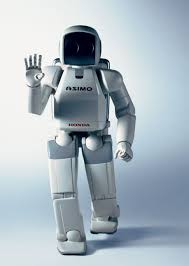
\includegraphics[scale=0.3]{asimo.jpg} 
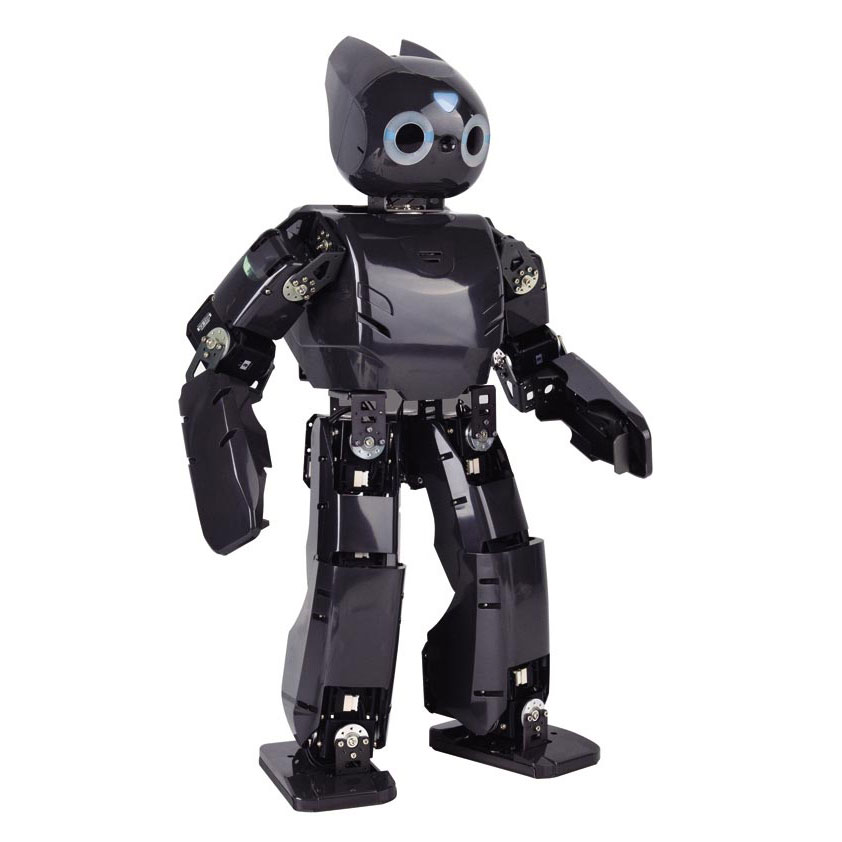
\includegraphics[scale=0.1]{Darwin_OP.jpg} 
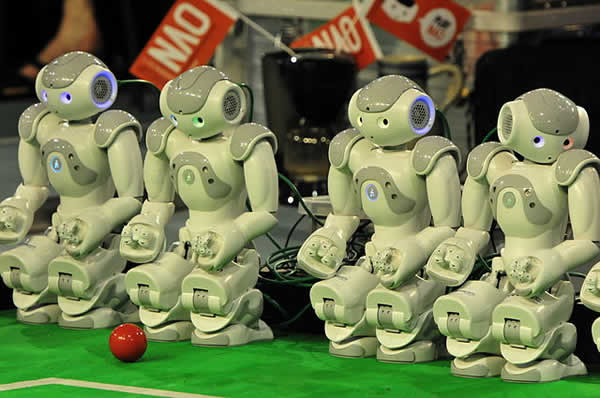
\includegraphics[scale=0.5]{13-06-28-robocup-eindhoven.jpg} 

\end{figure}
\end{frame}


\begin{frame}
  \frametitle{Introducci\'{o}n}
  \framesubtitle{Objetivo General}

  \begin{block}{Objetivo General}
	Dise\~nar y construir un robot humanoide capaz de detectar una pelota, buscarla y patearla con direcci\'on al arco, de forma aut\'onoma e inteligente.
   \end{block}
\end{frame}
\begin{frame}
  \frametitle{Introducci\'{o}n}
  \framesubtitle{Objetivos Espec\'{i}ficos}
  \begin{block}{Objetivos Espec\'{i}ficos}
  \begin{itemize}
    \item Dise\~no y ensamblaje
    \item Instalaci\'on y configuraci\'on de los componentes 
    \item Detecci\'on de la pelota
    \item Desplazamiento 
    \item Control de ca\'idas
    \item Comunicaci\'on entre controladores
    \item Aprendizaje por reforzamiento 
    \item Orientaci\'on al arco 
    \end{itemize}
  \end{block}
\end{frame}


  

\section{Construci\'on }
\begin{frame}
  \frametitle{Partes del robot}
  \framesubtitle{Piezas}

\begin{block}{Estructura}
	\begin{itemize}
		\item Con piezas de LEGO
		\item Desde cero
		\item Con el kit de piezas Bioloid
	\end{itemize}
\end{block}

 
\end{frame}

\begin{frame}
 \frametitle{Partes del robot}
 \framesubtitle{Piezas}
 
\begin{block}{Componentes utilizados del kit Bioloid}
\begin{itemize}
\item Motores Dynamixel
\item Bater\'ia de pol\'imero de litio
\item Giroscopio 
\end{itemize}
\end{block}

\begin{figure}[hbtp]
\centering
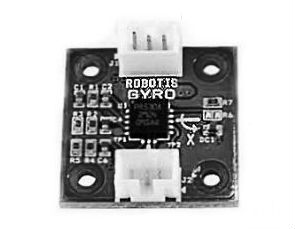
\includegraphics[scale=0.3]{gyro.jpg} 
\end{figure}

\end{frame}

\begin{frame}
 \frametitle{Partes del robot}
 \framesubtitle{Piezas}
 
\begin{block}{Componentes adicionales}
\begin{itemize}
\item Tarjeta controladora Arbotix
\item Raspberry Pi
\item C\'amara
\item Micro servo motores 
\item chip FTDI
\end{itemize}
\end{block}
\end{frame}

\begin{frame}
\frametitle{Partes del robot}
\framesubtitle{Ensamblaje}

\begin{block}{Modelo del robot}
	\begin{itemize}
		\item Modelo tipo B del manual	
	\end{itemize}
\end{block}

%\begin{block}{Desplazamiento}
%	\begin{itemize}
%	\item Escenas
%	\item Personal
%	\item Locaci\'{o}n
%\end{itemize}		
%\end{block}
\end{frame}

\begin{frame}
\frametitle{Partes del robot}
\framesubtitle{Conexiones}

%\begin{block}{Modelo del robot}
%	\begin{itemize}
%		\item Modelo tipo B del manual	
%	\end{itemize}
%\end{block}

\begin{figure}[hbtp]
\centering
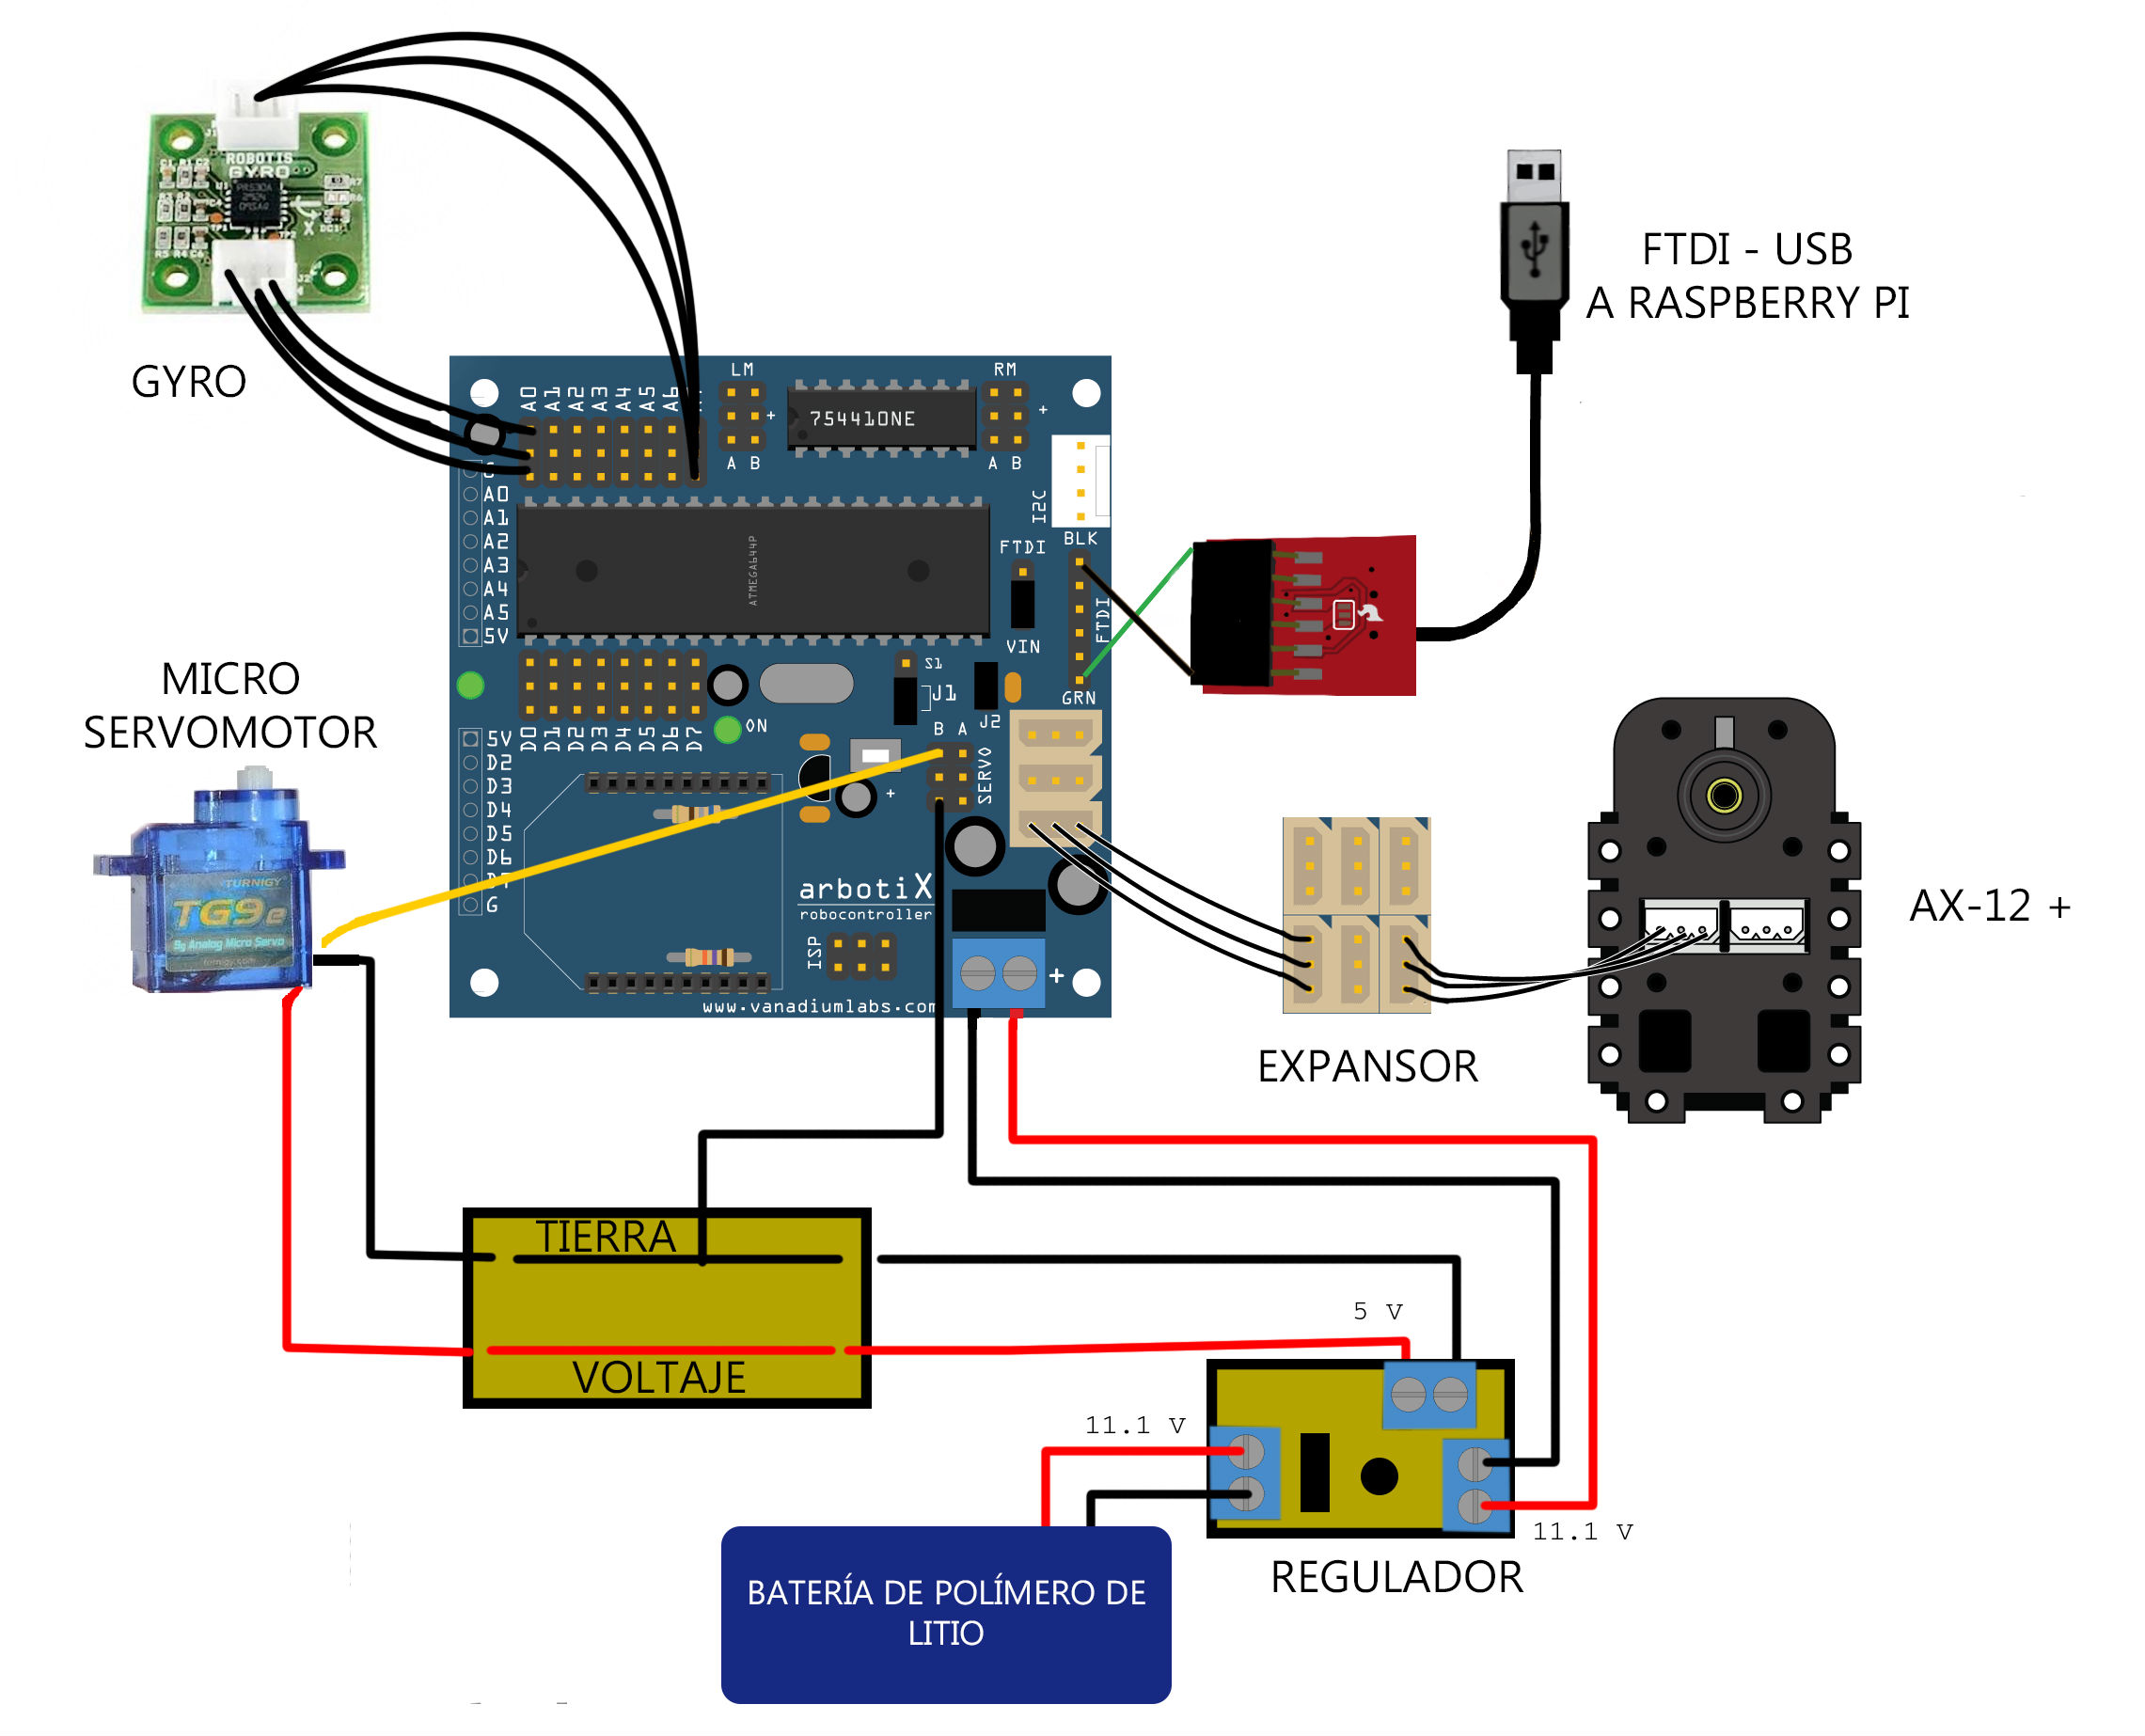
\includegraphics[scale=0.1]{arbotix_servo.jpg} 
\end{figure}

%\begin{block}{Desplazamiento}
%	\begin{itemize}
%	\item Escenas
%	\item Personal
%	\item Locaci\'{o}n
%\end{itemize}		
%\end{block}
\end{frame}

\begin{frame}
\frametitle{Detecci\'on de la pelota}

\begin{block}{Obtenci\'on de la imagen}
	\begin{itemize}
		\item Dificultades
		\item Soluci\'on	
	\end{itemize}
\end{block}

\begin{block}{Procesamiento de la imagen}
	\begin{itemize}
	\item De BGR a HSV
	\item Segmentaci\'on de regiones por color
	\item Filtros 
    \end{itemize}		
\end{block}

\end{frame}

\begin{frame}
\frametitle{Detecci\'on de la pelota}
\framesubtitle{Filtros: Ejemplo 1}

\begin{figure}[hbtp]
\centering
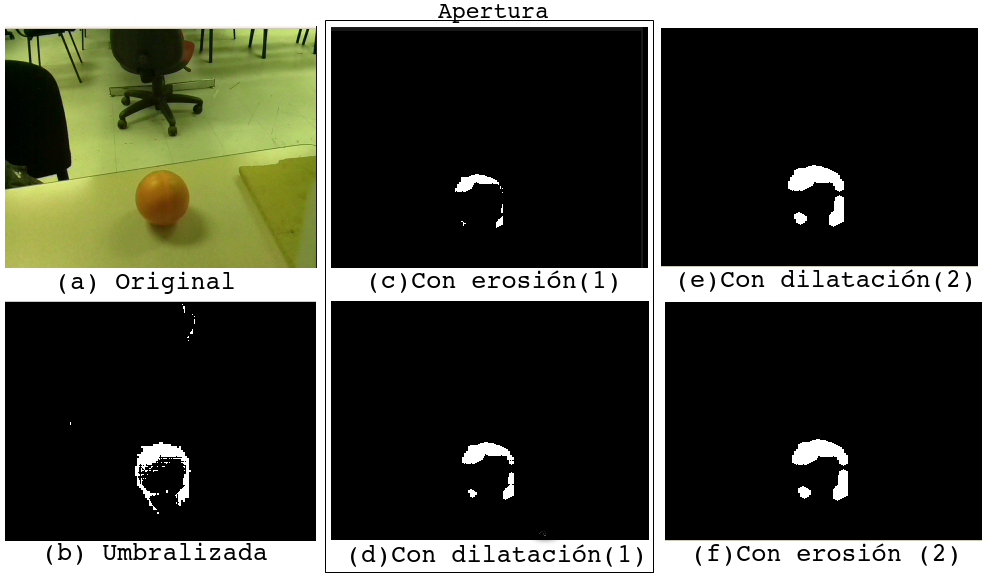
\includegraphics[scale=0.3]{filtros.png} 
\end{figure}

\end{frame}

\begin{frame}
\frametitle{Detecci\'on de la pelota}
\framesubtitle{Filtros: Ejemplo 2}

\begin{figure}[hbtp]
\centering
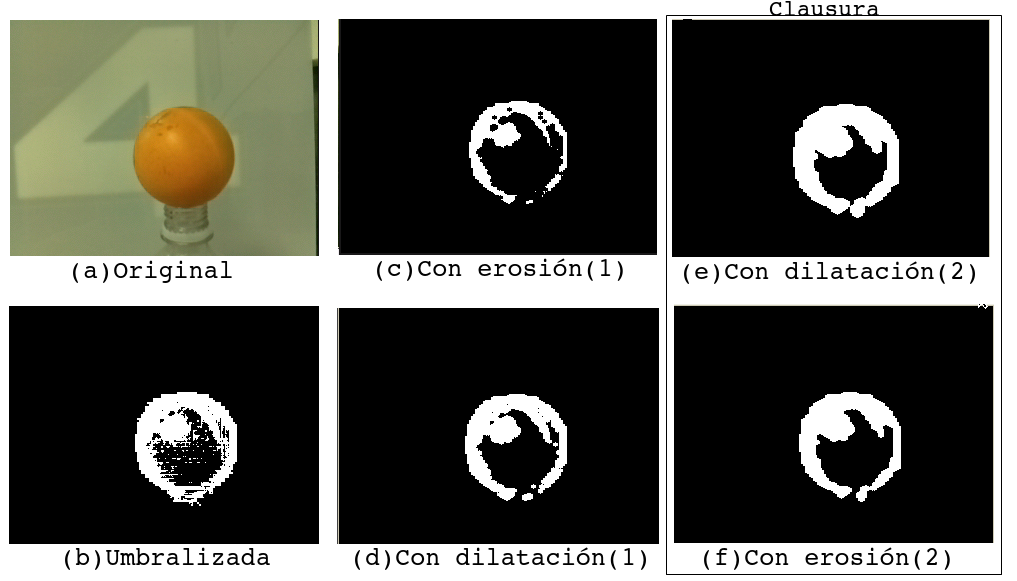
\includegraphics[scale=0.3]{conTodos4.png} 
\end{figure}

\end{frame}


\begin{frame}
\frametitle{Movimiento de las extremidades}

\begin{block}{Acciones de movimiento}
	\begin{itemize}
	\item Caminar hacia adelante
	\item Girar a la izquierda
	\item Girar a la derecha
	\item Levantarse desde la posición boca abajo
	\item Levantarse desde la posición boca arriba
	\item Patear con la pierna izquierda
	\item Patear con la pierna derecha
    \end{itemize}		
\end{block}

\end{frame}


\begin{frame}
\frametitle{Movimiento de la c\'amara}
\begin{figure}[hbtp]
\centering
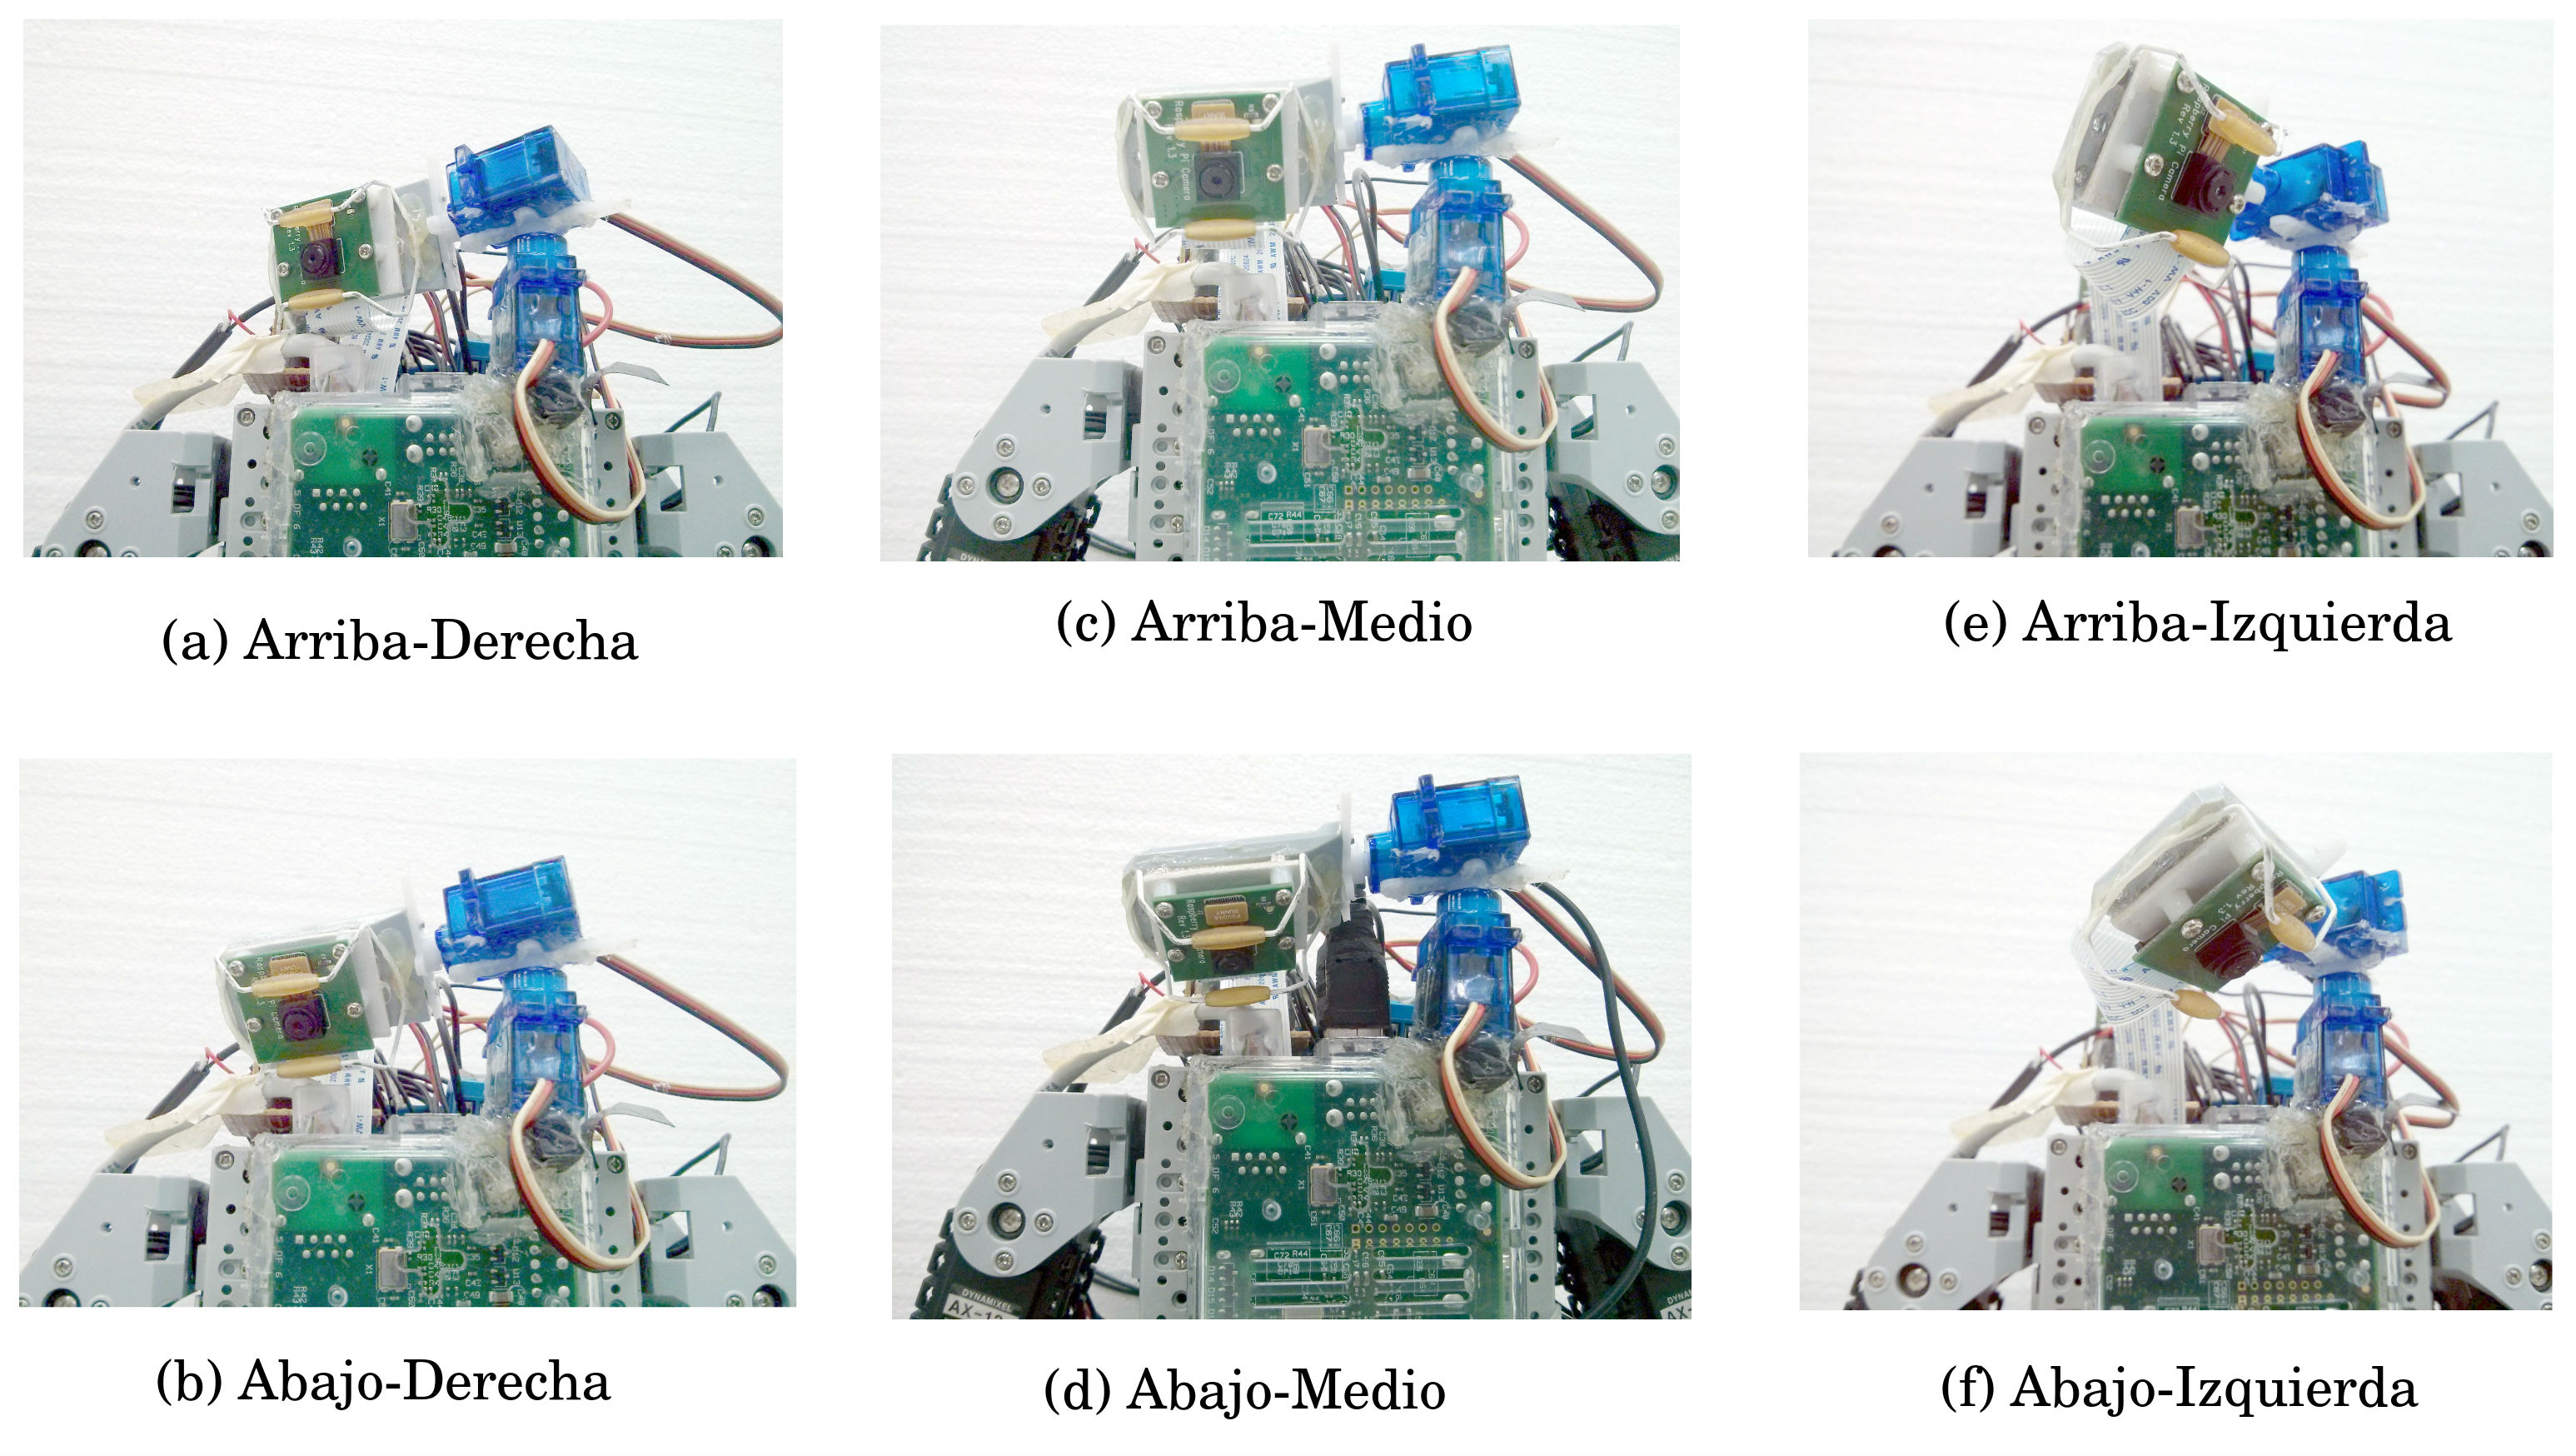
\includegraphics[scale=0.09]{posicionesCamara.jpg} 
\end{figure}
\end{frame}


\begin{frame}
\frametitle{Representaci\'on del mundo}
\begin{figure}[hbtp]
\centering
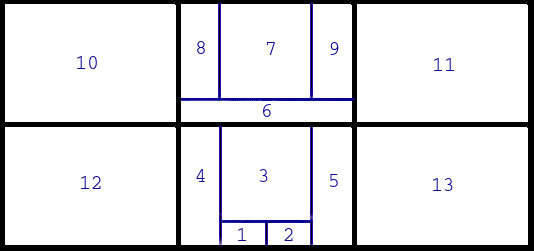
\includegraphics[scale=0.5]{Regiones.jpg} 
\end{figure}
\end{frame}



\begin{frame}
\frametitle{Comunicaci\'on Arbotix-Raspberry Pi}

\begin{itemize}
	\item Herramienta: ROS (Robot Operating System)
	\item Paradigma Cliente/Servidor
	\item Comunicaci\'on bidireccional y s\'incrona
\end{itemize}	

\end{frame}



\begin{frame}
\frametitle{Aprendizaje}

\begin{block}{Motivaci\'on}
\begin{itemize}
	\item Aprendizaje por reforzamiento
	\item Aprendizaje-Q
\end{itemize}
\end{block}	

\begin{block}{Modelo del problema}
\begin{itemize}
	\item Estados
	\item Acciones
	\item Recompensas
\end{itemize}
\end{block}	

\end{frame}


\begin{frame}
\frametitle{Modelo del problema}
\framesubtitle{Estados}
\begin{figure}[hbtp]
\centering
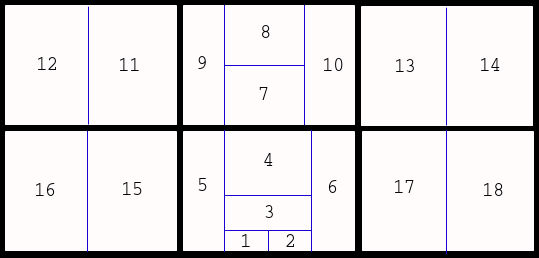
\includegraphics[scale=0.5]{Regiones2.jpg} 
\end{figure}
\end{frame}

\begin{frame}
\frametitle{Modelo del problema}
\framesubtitle{Acciones}

\begin{itemize}
 \item Caminar un paso hacia adelante
 \item Caminar dos pasos hacia adelante
 \item Caminar cuatro pasos hacia adelante
 \item Girar a la izquierda
 \item Girar doble a la izquierda
 \item Girar a la derecha
 \item Girar doble a la derecha
\end{itemize}

\end{frame}


\begin{frame}
\frametitle{Modelo del problema}
\framesubtitle{Recompensas}

\begin{equation}
R(s,a,s') = \dfrac{d(s) - d(s')}{10}
\end{equation}

\begin{figure}[hbtp]
\centering
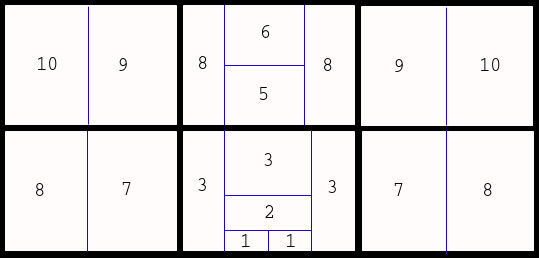
\includegraphics[scale=0.5]{Distancias2.jpg} 
\end{figure}

\end{frame}



\begin{frame}
\frametitle{Aprendizaje}

\begin{block}{Elecci\'on de la acci\'on}
\begin{equation}
 P(a_{i} | s) = \dfrac{k^{Q(s,a_{i})}}{\sum_{j}k^{Q(s,a_{j})}}
\end{equation}
\end{block} 

\begin{block}{Actualizaci\'on de Q(s,a)}
\begin{equation}
Q (s,a) = r + {\gamma\max_{a'}} Q(\delta(s ,a ) , a') 
\end{equation}
\end{block}

\end{frame}




\begin{frame}
\frametitle{Aprendizaje}
\framesubtitle{Detecci\'on de ca\'idas}

\begin{itemize}
 \item Velocidad angular (-300,300)
 \item Error estable (-80,100)
\end{itemize}

\begin{figure}[hbtp]
\centering
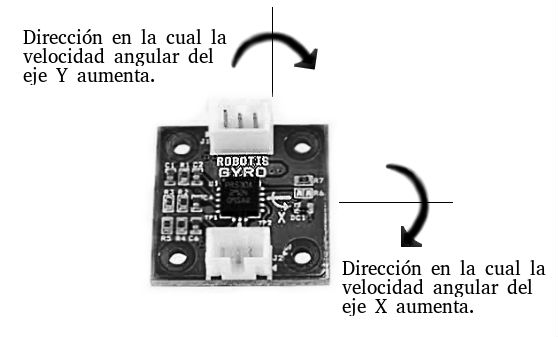
\includegraphics[scale=0.3]{gyroDireccion.jpg} 
\end{figure}

\end{frame}



\begin{frame}
\frametitle{Aprendizaje}
\framesubtitle{Orientaci\'on al arco}

\begin{figure}[hbtp]
\centering
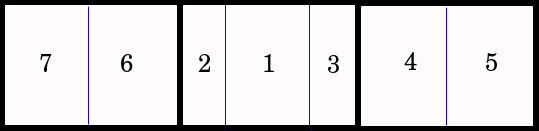
\includegraphics[scale=0.4]{RegionesArco.jpg} 
\end{figure}

\end{frame}


\section{Experimentos y Resultados}
\begin{frame}
  \frametitle{Experimentos}
  
  \begin{block}{Simples}
		\begin{itemize}
		\item Herradura
		\item Embobinado con cuerda
		\item Embobinado con cinta tubular
		\item Pasa 3 hala 2
 		\end{itemize}
	   \end{block}
\begin{block}{Compuestos}
	\begin{itemize}
		\item Lote estandar en cuerdas
		\item Equipo de Protecci\'{o}n Personal
	\end{itemize}
\end{block}
\end{frame}

\begin{frame}
\frametitle{Experimentos}
\begin{block}{Completos}
	\begin{itemize}
		\item Ascenso
		
	\end{itemize}
\end{block}
\end{frame}

\section{Conclusiones}
\begin{frame}
\frametitle{Conclusiones}
\begin{block}{Accesibilidad}

\end{block}


\end{frame}
\section{Recomendaciones}
\begin{frame}
\frametitle{Recomendaciones}
\begin{block}{Recomendaciones}

\end{block}
\end{frame}
\begin{frame}

\LARGE{PREGUNTAS}
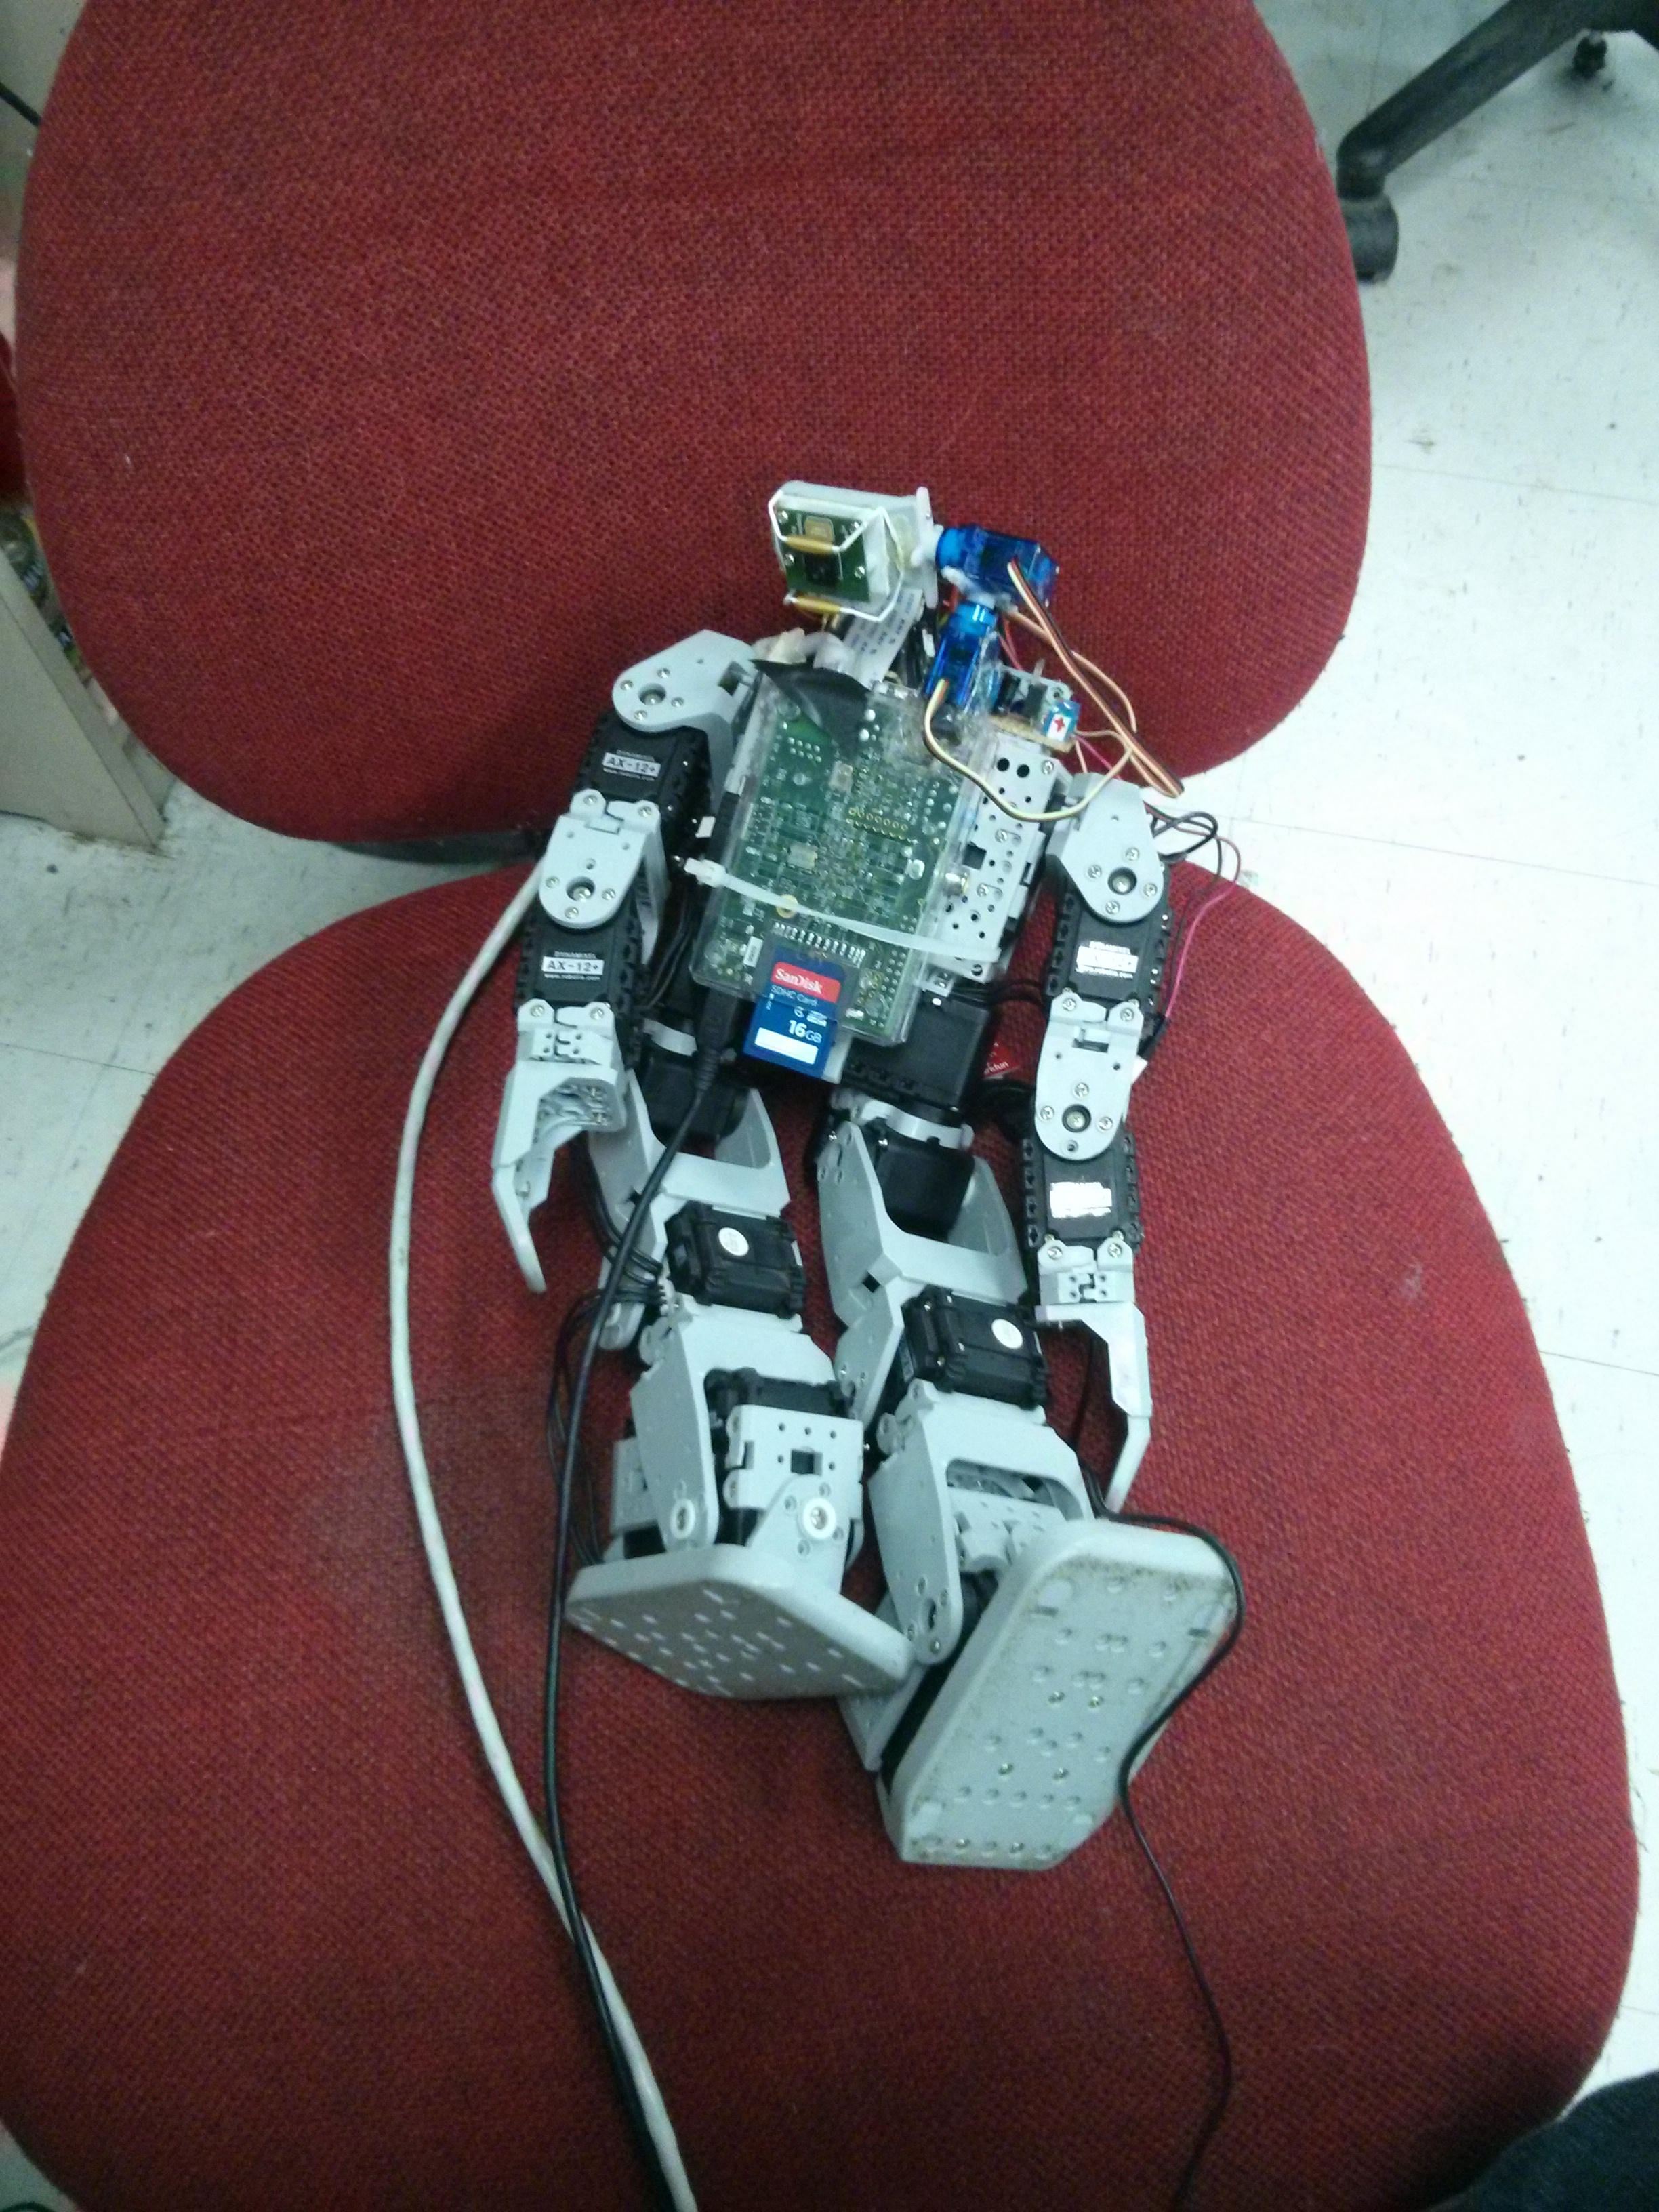
\includegraphics[scale=0.25]{tirolesa}
\end{frame}
\end{document}